\chapter{Arquitetura}
\begin{figure}[H]
	\centering
		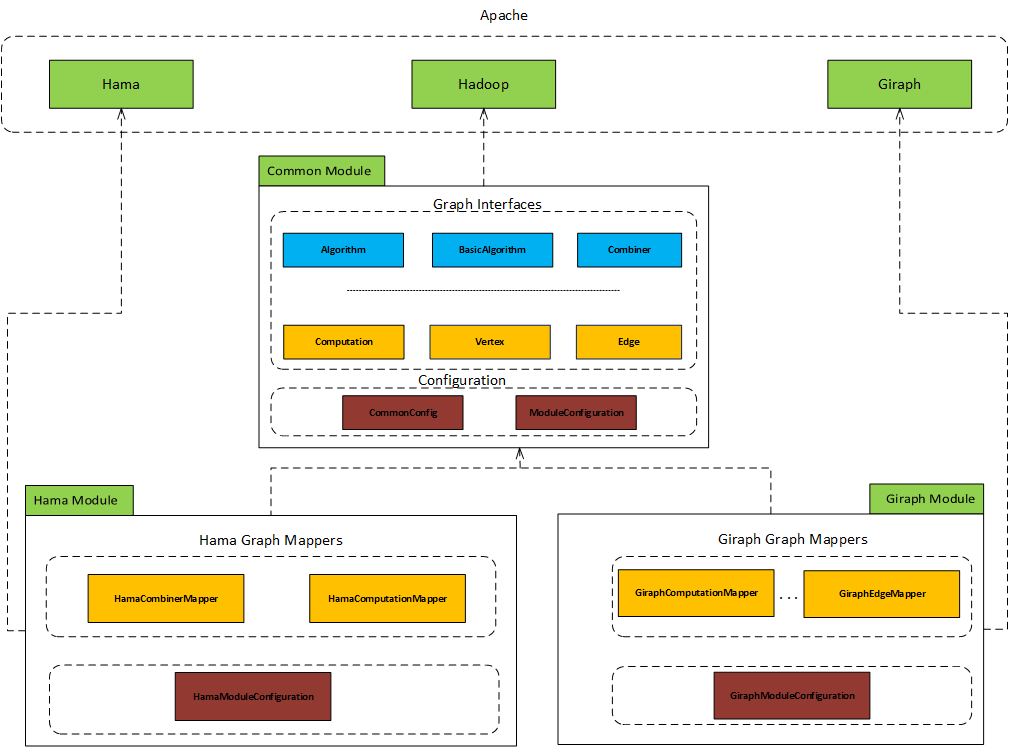
\includegraphics[width=\linewidth]{arquitetura}
	\caption{Em azul estão as interfaces e classes que devem ser implementadas por um programador que esteja interessado em implementar um algoritmo no módulo comum. As outras cores representam interfaces e classes que devem ser implementadas para criar-se um novo módulo sobre o módulo comum.}
	\label{fig:arquitetura}
\end{figure}

O módulo comum foi construído de modo a que se possa fazer proveito das interfaces programáveis disponibilizas pelas plataformas Apache Giraph e Apache Hama. Usando o módulo comum é possível usar tipos de mensagens e tipos de valor para vértices diferentes, mesmo usando a plataforma Apache Hama onde isto não é possível.

Para que se torne possível a utilização das interfaces disponibilizadas pelo módulo comum, criou-se um \texttt{CommonConfig} que tem a responsabilidade de registar as implementações comuns num \texttt{ModuleConfig}. Os módulos respetivos às plataformas, que estão a mapear para o módulo comum, têm de no \texttt{ModuleConfig} proceder às configurações necessárias para a respetiva plataforma. Esta implementação implica para que se use o módulo comum se proceda ao uso do CommonConfig.

Contudo, nem todas as funcionalidades são disponibilizas pelo módulo comum. Uma das funcionalidades que não foi conseguida até ao momento foi mapear os agregadores devido à diferença dos detalhes da sua implementação entre as duas plataformas. Apesar de não ser possível a implementação de agregadores comuns às duas plataformas, é possível utilizar agregadores cujo tipo do valor a agregar é diferente do tipo do valor do vértice, o que não era possível no Hama. Existe ainda outra funcionalidade que não foi mapeada, o \texttt{MasterCompute}, devido a não existir implementação no Hama. O \textit{input/output} é diferente nas duas plataformas daí que não exista nenhuma abstração no módulo comum.